% =============================================================================
%  FENS / IUS Bachelor Graduation Project Report
%  Project: Quantum-Enhanced Multi-Modal Vector Search
%  Build:   make           (uses pdflatex + bibtex via latexmk-free Makefile)
%  Edit:    chapters/*.tex and references.bib only. Do not change the preamble
%           without checking GUIDELINES.md first - template compliance matters.
% =============================================================================

\documentclass[12pt,a4paper,oneside]{report}

% -------- Fonts: Times-equivalent for both text and math -----------------------
\usepackage[T1]{fontenc}
\usepackage[utf8]{inputenc}
\usepackage{mathptmx}                       % Times Roman text + math

% -------- Page geometry per FENS template (4cm L, 3cm B, 2.5cm T/R) -----------
\usepackage[a4paper,left=4cm,right=2.5cm,top=2.5cm,bottom=3cm]{geometry}

% -------- Line spacing 1.5 ----------------------------------------------------
\usepackage{setspace}
\onehalfspacing

% -------- Paragraphs: indented first line + 12pt spacing ----------------------
\usepackage{parskip}
\setlength{\parindent}{1.27cm}
\setlength{\parskip}{12pt plus 1pt minus 1pt}

% -------- Common typesetting tools --------------------------------------------
\usepackage{graphicx}
\graphicspath{{figures/}}
\usepackage{caption}
\captionsetup{font=small,labelfont=bf,justification=centering}
\usepackage{booktabs}                       % proper table rules
\usepackage{array}
\usepackage{amsmath,amssymb,amsthm}
\usepackage{mathtools}                      % \coloneqq and friends
\usepackage{braket}                         % \ket{}, \bra{} for quantum notation
\usepackage{siunitx}                        % \SI{}, numeric formatting
\usepackage{microtype}                      % subtle kerning, no visible change
\usepackage{enumitem}
\usepackage{xcolor}
\usepackage{listings}                       % code blocks if needed
\usepackage{tabularx}
% Coloured, clickable hyperlinks. Single muted blue across internal references,
% citations, and URLs. Color must be defined BEFORE hyperref is loaded.
\definecolor{iuslink}{HTML}{1E40AF}
\usepackage[%
  colorlinks=true,
  linkcolor=iuslink,
  citecolor=iuslink,
  urlcolor=iuslink,
  filecolor=iuslink,
]{hyperref}
\usepackage{url}

% -------- IEEE citation style (numeric, [1], [2,3,4]) -------------------------
\usepackage[numbers,sort&compress]{natbib}
\bibliographystyle{IEEEtran}

% -------- Chapter heading formatting ------------------------------------------
\usepackage{titlesec}
\titleformat{\chapter}[block]
  {\normalfont\Large\bfseries}{\thechapter.}{0.5em}{\Large\MakeUppercase}
\titlespacing*{\chapter}{0pt}{0pt}{18pt}

% -------- TOC dot leaders for every level (default report class omits dots
%          on chapter rows; we want them everywhere for the FENS template). ---
\usepackage{tocloft}
\renewcommand{\cftchapleader}{\cftdotfill{\cftdotsep}}
\renewcommand{\cftchapdotsep}{\cftdotsep}

% Prefix List-of-Tables / List-of-Figures entries with "Table N:" / "Figure N:"
% so they read literally as "Table 1: Caption..." in the rendered PDF.
\renewcommand{\cfttabpresnum}{Table~}
\renewcommand{\cfttabaftersnum}{:}
\setlength{\cfttabnumwidth}{5.5em}
\setlength{\cfttabindent}{0pt}

\renewcommand{\cftfigpresnum}{Figure~}
\renewcommand{\cftfigaftersnum}{:}
\setlength{\cftfignumwidth}{5.5em}
\setlength{\cftfigindent}{0pt}

% -------- Sequential numbering for tables/figures/equations across the whole
%          document (no chapter prefix, so we get "Table 1" instead of
%          "Table 3.1" per the FENS template examples). --------------------
\usepackage{chngcntr}
\counterwithout{figure}{chapter}
\counterwithout{table}{chapter}
\counterwithout{equation}{chapter}

% -------- TOC / list-of styling -----------------------------------------------
\renewcommand{\contentsname}{TABLE OF CONTENTS}
\renewcommand{\listfigurename}{LIST OF FIGURES}
\renewcommand{\listtablename}{LIST OF TABLES}
\renewcommand{\bibname}{REFERENCES}

% -------- Project-wide constants (single source of truth for the cover) -------
\newcommand{\ProjectTitle}{Quantum-Enhanced Multi-Modal Vector Search: A Hybrid Database Web App}
\newcommand{\ProjectShortTitle}{Quantum-Enhanced Multi-Modal Vector Search}
\newcommand{\Supervisor}{Assist.\,Prof.\,Dr. Ali Abd Almisreb}
\newcommand{\InstitutionName}{International University of Sarajevo}
\newcommand{\FacultyName}{Faculty of Engineering and Natural Sciences}
\newcommand{\SubmissionMonthYear}{\ifcase\month\or January\or February\or March\or April\or May\or June\or July\or August\or September\or October\or November\or December\fi{} \the\year}

% =============================================================================
\begin{document}

% ============================  FRONT MATTER  =================================
% Roman numerals iii ... onwards per template; cover counts but is not numbered.
\pagenumbering{roman}
\setcounter{page}{1}

% Cover page. Do not number this page.
\thispagestyle{empty}

\begin{center}
{\Large\bfseries \MakeUppercase{\ProjectTitle}\par}

\vspace{2cm}

% Place the IUS logo at figures/ius_logo.png. Until then, this falls back to
% the placeholder so the build never breaks.
\IfFileExists{figures/ius_logo.png}{%
  
\includegraphics[height=4cm]{figures/ius_logo.png}%
}{%
  \fbox{\parbox{4cm}{\centering\vspace{1.5cm}IUS LOGO\\\texttt{figures/ius\_logo.png}\vspace{1.5cm}}}%
}

\vspace{2cm}

{\large
Elhan Mahmutovic\\
Adna Kikanovic\\
Adnan Musanovic\\
Mirza Abdulahovic\par}

\vspace{2cm}

{\large \MakeUppercase{\InstitutionName}\par}

\vspace{1cm}

{\large \the\year\par}

\vfill
\end{center}

\clearpage

% Inner title page (per FENS template).
\thispagestyle{empty}
\begin{center}
{\Large\bfseries \MakeUppercase{\ProjectTitle}\par}

\vspace{2cm}

{\large BY\par}

\vspace{1cm}

{\large
Elhan Mahmutovic\,--\,Software Engineering\\
Adna Kikanovic\,--\,Software Engineering\\
Adnan Musanovic\,--\,Software Engineering\\
Mirza Abdulahovic\,--\,Software Engineering\par}

\vspace{2cm}

A graduation project submitted in partial fulfillment of the\\
requirements for the degree of Bachelor of Science at the\\
\FacultyName\\
\InstitutionName

\vspace{2cm}

{\SubmissionMonthYear}
\end{center}
\clearpage

\chapter*{APPROVAL PAGE}
\addcontentsline{toc}{chapter}{APPROVAL PAGE}

I certify that I have supervised and read this study and that in my opinion, it conforms to acceptable standards of scholarly presentation and is fully adequate, in scope and quality, as a graduation project for the degree of Bachelor of Science at the \FacultyName.

\vspace{2cm}

% Mentor block, right-aligned per FENS template.
\begin{flushright}
\makebox[8cm][l]{\dotfill}\\
\Supervisor\\
\emph{Mentor}
\end{flushright}

\clearpage

\chapter*{DECLARATION}
\addcontentsline{toc}{chapter}{DECLARATION}

We hereby declare that all information in this document has been obtained and presented in accordance with academic rules and ethical conduct. We also declare that, as required by these rules and conduct, we have fully cited and referenced all material and results that are not original to this work.

\vspace{1.5cm}

% \SigRow renders one signature line. Signature label + dotted line are pushed
% to the right; the name stays on the left.
\newcommand{\SigRow}[1]{%
  \noindent #1 \hfill Signature \makebox[6cm][l]{\dotfill}\par
  \vspace{1.2cm}%
}

\SigRow{Elhan Mahmutovic}
\SigRow{Adna Kikanovic}
\SigRow{Adnan Musanovic}
\SigRow{Mirza Abdulahovic}

\vspace{0.5cm}
\hfill Date \makebox[4cm][l]{\dotfill}

\vspace{2cm}
\begin{center}\MakeUppercase{\InstitutionName}\end{center}

\clearpage

\chapter*{DECLARATION OF COPYRIGHT AND AFFIRMATION OF FAIR USE OF UNPUBLISHED WORK}
\addcontentsline{toc}{chapter}{DECLARATION OF COPYRIGHT}

\noindent Copyright \textcopyright{} \the\year{} by Elhan Mahmutovi\'{c}, Adna Kikanovi\'{c}, Adnan Mu\v{s}anovi\'{c}, and Mirza Abdulahovi\'{c}. All rights reserved.

\vspace{1em}
\noindent\textbf{\ProjectTitle}

\vspace{1em}
\noindent No part of this unpublished work may be reproduced, stored in a retrieval system, or transmitted, in any form or by any means, electronic, mechanical, photocopying, recording or otherwise without prior written permission of the copyright holder and IUS Library.

\vspace{1.5em}
\noindent Affirmed by:

\vspace{1em}

% Same signature row as DECLARATION: name left, dotted line right.
\newcommand{\SigRowC}[1]{%
  \noindent #1 \hfill Signature \makebox[6cm][l]{\dotfill}\par
  \vspace{1.2cm}%
}

\SigRowC{Elhan Mahmutovi\'{c}}
\SigRowC{Adna Kikanovi\'{c}}
\SigRowC{Adnan Mu\v{s}anovi\'{c}}
\SigRowC{Mirza Abdulahovi\'{c}}

\vspace{0.5cm}
\hfill Date \makebox[4cm][l]{\dotfill}

\clearpage

\chapter*{ACKNOWLEDGEMENTS}
\addcontentsline{toc}{chapter}{ACKNOWLEDGEMENTS}

% TODO: write a short paragraph thanking the supervisor, the faculty, and anyone
% who supported the project. Keep it sincere and brief - one paragraph is plenty.

[ACKNOWLEDGEMENTS TEXT \,--\, see GUIDELINES.md \S Acknowledgements]

\clearpage

\chapter*{LIST OF ABBREVIATIONS}
\addcontentsline{toc}{chapter}{LIST OF ABBREVIATIONS}

% Keep this list alphabetical. Every acronym used in the body MUST appear here AND
% be expanded on first use in the text. See GUIDELINES.md \S Acronyms.

\begin{tabbing}
\hspace{3.5cm}\=\kill
AI         \> Artificial Intelligence \\
API        \> Application Programming Interface \\
CLIP       \> Contrastive Language\,--\,Image Pre-training \\
CPU        \> Central Processing Unit \\
FAISS      \> Facebook AI Similarity Search \\
GPU        \> Graphics Processing Unit \\
HNSW       \> Hierarchical Navigable Small World \\
IBM QPU    \> IBM Quantum Processing Unit \\
MRR        \> Mean Reciprocal Rank \\
NISQ       \> Noisy Intermediate-Scale Quantum \\
qRAM       \> Quantum Random-Access Memory \\
SDG        \> Sustainable Development Goal \\
SQL        \> Structured Query Language \\
ViT        \> Vision Transformer \\
\end{tabbing}

\clearpage


% Front-matter lists
\tableofcontents
\clearpage
\chapter*{ABSTRACT}
\addcontentsline{toc}{chapter}{ABSTRACT}

\begin{center}\textbf{\MakeUppercase{\ProjectTitle}}\end{center}

% 250-500 words. Cover: (1) problem, (2) methods, (3) results, (4) implications.
% Write this LAST, after the rest of the report has stabilised. See GUIDELINES.md
% \S Abstract for the structure to follow.

Vector search, the task of finding the stored items whose embeddings lie closest
to a query, underlies modern retrieval systems, including cross-modal search that
retrieves images from a text description. Two quantum primitives, Grover's
algorithm for unstructured search and the swap test for state similarity, appear
well suited to this task. This project investigates, through direct measurement,
whether they are of practical use for cross-modal vector search at the scale and
on the hardware available today.

We built a single framework in which classical, quantum, and hybrid search
engines answer the same queries over the same CLIP embeddings, so their rankings
can be compared on identical terms. Seven engines were implemented behind a
common interface: three classical baselines (an exact scan, an exact FAISS index,
and an approximate Hierarchical Navigable Small World graph), three quantum
engines (a swap-test estimator and two variants of Grover's algorithm), and a
hybrid that uses the classical index to shortlist candidates and the swap test to
rerank them. We benchmarked every engine over a controlled twenty-image
cross-modal dataset across a range of embedding dimensions and measurement shot
counts, recording retrieval accuracy as Mean Reciprocal Rank alongside
hardware-independent cost measures such as oracle calls, qubit count, and circuit
depth. The quantum engines ran on a classical simulator, with a single small
validation run on real IBM quantum hardware.

The results show that retrieval accuracy was governed by the embedding dimension
rather than by whether an engine was quantum. The swap test reproduced the
classical ranking accuracy once given a sufficient measurement budget, matching it
exactly at the highest dimension, and our Grover implementation reproduced its
theoretical oracle-call count exactly. No engine that performed its search
quantumly outperformed the classical graph-based baseline, however, and the
hybrid engine matched that baseline only because the classical index performed the
search. The underlying reason is structural: vector retrieval is dominated by
reading the dataset, a data-bound task, whereas quantum advantage concentrates on
compute-bound problems over small inputs. We conclude that cross-modal vector
search is not a natural fit for quantum methods, even setting aside the maturity
of current hardware, and that the apparent speed-up of quantum search rests on a
data-loading cost that the headline figures omit. The contribution of this work is
an honest, reproducible, like-for-like comparison and an explicit account of where
the quantum-classical gap actually lies.

\vspace{1em}
\noindent\textbf{Keywords:} \emph{quantum computing, vector search, similarity search, swap test, Grover's algorithm, CLIP, benchmarking}

\clearpage

\listoftables
\clearpage
\listoffigures
\clearpage

% ============================  MAIN MATTER  ==================================
\pagenumbering{arabic}
\setcounter{page}{1}

\chapter{INTRODUCTION}
\label{ch:introduction}

% Purpose (from template): tell the reader WHY this study exists. Start broad,
% narrow to the research question. Define terms on first use. Reference prior work.
%
% Target length: ~600-900 words for this chapter (project is 5,000-10,000 total).
% See report/STRUCTURE.md for the full per-section budget.

Modern machine-learning systems represent text, images, and other media as
high-dimensional vectors called embeddings, arranged so that items with similar
meaning sit close together in the vector space. Searching a collection then
reduces to finding the stored vectors nearest to a query vector, a task known as
vector search. It underlies image search, recommendation systems, and the
retrieval step of retrieval-augmented language models. When the query and the
stored items are different kinds of media, such as retrieving images from a
written description, the task is cross-modal retrieval, and it becomes tractable
once a single embedding model places both modalities in one shared space.

Quantum computing offers two primitives that appear, at first sight, well matched
to this task. Grover's algorithm finds a marked item in an unstructured
collection using far fewer queries than a classical scan, and the swap test
estimates how similar two quantum states are. This study asks, through
measurement rather than assertion, whether those primitives are of practical use
for cross-modal vector search at the scale and on the hardware available today.
It is an investigation of where quantum search does and does not fit, not an
attempt to demonstrate a quantum advantage.

\section{Background of Study}
\label{sec:background}

% What is vector search, what is cross-modal retrieval, what is CLIP, and what
% does "quantum similarity" mean here. Two or three paragraphs. Cite the
% foundational papers (CLIP, Grover, Buhrman et al. swap test).

An embedding model maps an input to a fixed-length vector so that semantically
related inputs map to nearby vectors. For cross-modal retrieval we use CLIP, a
model trained on a large collection of image and caption pairs to place an image
and its description close together in a shared
space~\cite{radford2021clip}. Once both a text query and a set of images live in
that space, answering the query means ranking the image vectors by their
closeness to the query vector. The simplest way to do this is an exhaustive scan
that compares the query against every stored vector, which costs $O(N)$
comparisons for $N$ items. Production systems reduce this cost with specialised
libraries such as FAISS, which performs the exact scan
efficiently~\cite{johnson2019faiss}, or with approximate methods such as the
Hierarchical Navigable Small World (HNSW) graph, which reaches a near neighbour
in roughly $O(\log N)$ steps by navigating a layered proximity
graph~\cite{malkov2020hnsw}.

The quantum side of the comparison rests on two ideas. Grover's algorithm
searches an unstructured collection of $N$ items for a marked one using only
about $\sqrt{N}$ queries to an oracle, a quadratic improvement over the linear
classical scan~\cite{grover1996}. The swap test takes two quantum states and
estimates the squared overlap between them from a single measured
qubit~\cite{buhrman2001swaptest}; because a normalised embedding can be encoded
in the amplitudes of a quantum state, that overlap is a similarity score. Both
techniques therefore have a natural reading as vector-search operations, Grover
as the search itself and the swap test as the similarity comparison.

The difficulty is that these speed-ups assume the data is already available
inside the quantum computer. For Grover to search real vectors, an oracle would
have to recognise the closest item while the whole dataset is held in
superposition, which requires a quantum random-access memory that does not yet
exist at usable scale; loading the data one item at a time instead costs $O(N)$
and removes the very advantage the algorithm promises~\cite{aaronson2015readfine}.
This tension between an algorithm's asymptotic promise and the cost of getting
data into the machine is the central question the study examines.

\section{Problem Statement and Research Aims}
\label{sec:problem}

% Make the gap explicit: classical vector search is well-studied; the practical
% relevance of quantum vector search at NISQ scale is not. State what we set out
% to MEASURE - not what we set out to PROVE.

Classical vector search is mature, fast, and well understood. Whether quantum
methods add anything to it at the scale available today is far less clear, and
popular accounts often overstate the case. The gap this work addresses is
empirical: there are few honest, like-for-like comparisons that run classical and
quantum similarity search on the same data and report both retrieval accuracy and
the resources each method consumes. We built such a comparison. A single common
interface lets classical, quantum, and hybrid engines answer the same queries
over the same embeddings, so their rankings can be placed side by side and scored
identically.

We frame the work as a measurement rather than a proof of advantage. Present-day
devices are small and noisy, the regime usually called noisy intermediate-scale
quantum (NISQ), so we run the quantum engines mostly on a classical simulator and
validate the hardware path with a single small run on a real quantum processor.
The goal is to determine, on a controlled cross-modal dataset, how the quantum
and hybrid engines compare with strong classical baselines, and to state plainly
the conditions under which each approach is preferable.

\section{Research Questions and Objectives}
\label{sec:questions}

% List 3-4 measurable research questions. Each must map to something the
% benchmark harness already produces (MRR, oracle calls, circuit depth, etc.)
% so we never write a question we cannot answer with data we already have.

\begin{enumerate}[label=RQ\arabic*., leftmargin=*]
  \item \emph{Accuracy:} Does swap-test similarity reproduce the ranking of
        classical cosine similarity, and what is the shot budget required to do so?
  \item \emph{Scaling:} Does our Grover implementation reproduce the
        $\lfloor \pi\sqrt{N}/4 \rfloor$ oracle-call scaling in practice?
  \item \emph{Practicality:} Under what conditions \,--\, if any \,--\, would a
        quantum vector-search engine outperform a production classical baseline
        (HNSW) on the same dataset?
  \item \emph{Suitability:} Independent of hardware maturity, is cross-modal
        vector search a problem class that quantum computing is suited to, given
        that quantum advantage concentrates on compute-bound problems over small
        data rather than data-bound retrieval?
\end{enumerate}

To answer these questions we set four objectives, each corresponding to a
concrete artefact in the project repository:

\begin{enumerate}[leftmargin=*]
  \item Implement a suite of search engines spanning classical, quantum, and
        hybrid approaches behind a single common interface, so that one query can
        be answered by any of them and the results compared directly.
  \item Build a reproducible benchmark harness and a controlled cross-modal
        dataset, and collect a complete set of results across embedding
        dimensions and measurement shot counts.
  \item Provide a web application that displays the engines' rankings side by
        side for inspection.
  \item Produce an honest written analysis that answers the research questions
        from the measured data, including the cases where quantum methods do not
        help.
\end{enumerate}

\chapter{LITERATURE REVIEW}
\label{ch:literature}

% Focused review. Do NOT write a history of quantum computing. The committee is
% not made of quantum experts (see project brief), so explain just enough for a
% CS-bachelor reader to follow the methodology chapter.
% Target length: ~800-1,200 words.

\section{Classical Vector Search}
\label{sec:lit:classical}

% Cover, in order of complexity: exact brute force, FAISS flat indices,
% approximate-nearest-neighbour graphs (HNSW). Frame HNSW as the production
% standard - it is the most important comparison point on slide 11 of the
% midterm deck.

% Example sentence that exercises the citation machinery -- rewrite, but keep
% the same citation pattern so the reference list stays populated.
Exact nearest-neighbour search at scale was popularised by FAISS, a SIMD-vectorised
library for billion-scale similarity search~\cite{johnson2019faiss}. For datasets
where exact search is too expensive, the de facto approximate method is the
Hierarchical Navigable Small World graph~\cite{malkov2020hnsw}, which trades a
small recall loss for $O(\log N)$ retrieval.

[CLASSICAL VECTOR SEARCH \,--\, expand the paragraph above; add a brute-force
baseline reference if one is wanted.]

\section{Cross-Modal Embeddings}
\label{sec:lit:embeddings}

% One short subsection on CLIP. Explain contrastive learning at a high level
% and why text and image embeddings end up in the same metric space.

CLIP aligns a text encoder and an image encoder via contrastive pre-training
on 400~million image--caption pairs, producing a shared 512-dimensional space in
which cosine similarity captures cross-modal relevance~\cite{radford2021clip}.

[CLIP / CROSS-MODAL EMBEDDINGS \,--\, expand: explain ViT-B/32, mention that
we truncate the 512-dim output to 64/128/256 for benchmarking.]

\section{Quantum Similarity Primitives}
\label{sec:lit:quantum}

% Swap test (Buhrman et al.), amplitude encoding state preparation, Grover.
% Be honest about what is "speedup" and what is "amortised state preparation
% cost" - the qRAM caveat goes here, not in the methodology.

Grover's algorithm provides a quadratic speedup for unstructured
search~\cite{grover1996}. The swap test, introduced by Buhrman et
al.~\cite{buhrman2001swaptest}, estimates the squared inner product of two
quantum states with a single ancilla measurement. Both algorithms assume
that the dataset is already encoded into a quantum state; in the absence of
quantum RAM~\cite{giovannetti2008qram}, this state preparation step costs
$O(N)$ and cancels Grover's quadratic advantage at the system
level~\cite{aaronson2015readfine}.

[QUANTUM PRIMITIVES \,--\, expand: explain amplitude encoding cost, give the
formula for swap-test overlap, foreshadow the qRAM discussion in chapter~4.]

\section{Hybrid Classical--Quantum Architectures}
\label{sec:lit:hybrid}

% Brief discussion of recent hybrid retrieval pipelines that use a classical
% prefilter and a quantum reranker. Frame our hybrid_hnsw_swap_test engine as
% an instance of this pattern.

Quantum machine-learning surveys~\cite{biamonte2017qml} catalogue hybrid
classical--quantum pipelines that delegate the expensive global step to
classical hardware and reserve quantum resources for a smaller, structured
subproblem. Our \texttt{hybrid\_hnsw\_swap\_test} engine follows this pattern:
HNSW returns a small candidate pool, then the swap test reranks it on the
simulator (implemented with Qiskit~\cite{qiskit2024}).

[HYBRID ARCHITECTURES \,--\, expand: discuss other hybrid retrieval approaches
in the literature; position our work as an instance of this pattern.]

\chapter{RESEARCH METHODOLOGY}
\label{ch:methodology}

% Describe how the study was conducted, well enough for someone else to
% reproduce it. This chapter is the bulk of the report (~1,500-2,500 words).
% The "Use of AI Tools" subsection at the END is MANDATORY per handbook \S1.1.

\section{System Overview}
\label{sec:method:overview}

% One paragraph describing the modular monolith - data loader, embedding
% pipeline, engines, storage, API+UI. Reference Figure \ref{fig:architecture}.

The system is a modular monolith that performs cross-modal retrieval: given a
short text query such as ``a dog on a beach'', it returns the dataset images
whose content best matches that description. Text and images are never compared
directly. Instead, the same embedding model maps both into a shared vector
space, and retrieval becomes the problem of finding the dataset vectors closest
to the query vector. The defining property of the system is that the component
performing this closest-vector search is interchangeable. A classical engine, a
quantum engine, and a hybrid of the two all expose one common interface, so a
single query can be answered by any of them and the rankings placed side by
side. This makes the system an instrument for comparing search strategies
rather than a single retrieval product.\footnote{The full source code, benchmark
harness, and dataset configuration are publicly available at
\url{https://github.com/Mirza404/quantum-vector-search}.}

This interchangeability is enforced by a single design decision that runs
through the whole codebase: the strategy pattern. Each stage of the pipeline is
defined by an abstract interface, and concrete implementations plug into it.
Data loaders implement \texttt{BaseDataLoader}, embedding models implement
\texttt{EmbeddingGenerator}, and every search engine implements
\texttt{SearchEngineStrategy}, which requires just two operations,
\texttt{build\_index} and \texttt{search}. Because all engines satisfy the same
contract, the surrounding harness that loads data, generates embeddings, runs
queries, and records results is identical for every engine. Any difference we
measure between a classical and a quantum engine therefore reflects the engine
itself, not the code around it. Which engines run, at which vector dimensions,
and with how many measurement shots is selected in a configuration file
(\texttt{benchmarks.yaml}) rather than by editing source, so an experiment is
defined by configuration rather than by code changes.

The pipeline is organised into five phases, shown in
Figure~\ref{fig:architecture}. In the first phase, data loading, a
\texttt{DirectoryDataLoader} reads the image files and the accompanying
ground-truth pairs that define which image each query should retrieve. In the
second phase, the embedding pipeline, a CLIP model converts every image and
every text query into a vector. In the third phase the search engines build
their indexes over these vectors and answer queries, each engine applying its
own strategy, whether classical, quantum, or hybrid. In the fourth phase the
outcome of every run, including its accuracy and resource measurements, is
written to a PostgreSQL database. The fifth phase exposes the system through a
FastAPI backend and a React interface, which lets a user issue a query and
inspect the rankings returned by each engine. The sections that follow describe
each phase in turn: the dataset and ground truth in
Section~\ref{sec:method:dataset}, the embedding pipeline in
Section~\ref{sec:method:embeddings}, and the individual search engines in
Section~\ref{sec:method:engines}.

\begin{figure}[ht]
  \centering
  \begin{tikzpicture}[
      font=\small,
      box/.style={draw, rounded corners, align=center, inner sep=5pt,
        text width=58mm, fill=gray!8},
      eng/.style={draw, rounded corners, align=center, inner sep=4pt,
        text width=30mm, minimum height=12mm, font=\footnotesize},
      classical/.style={eng, fill=blue!10, draw=blue!55},
      quantum/.style={eng, fill=violet!12, draw=violet!55},
      hybrid/.style={eng, fill=green!12, draw=green!50!black!70},
      arr/.style={-{Latex[length=2.2mm]}, semithick}
    ]
    \node[box] (load) {\textit{Phase 1: Data loading}\\[2pt]
      \textbf{DirectoryDataLoader}\\ images and ground-truth pairs};
    \node[box, below=7mm of load] (embed) {\textit{Phase 2: Embedding}\\[2pt]
      \textbf{CLIPEmbeddingModel}\\ ViT-B/32, one vector per image and query};
    \node[box, below=7mm of embed] (strategy) {\textit{Phase 3: Search engines}\\[2pt]
      \textbf{SearchEngineStrategy}\\ \texttt{build\_index} / \texttt{search}};

    \node[quantum, below=11mm of strategy] (qu) {\textbf{Quantum}\\ swap test, Grover};
    \node[classical, left=5mm of qu] (cl) {\textbf{Classical}\\ brute force, FAISS flat, FAISS HNSW};
    \node[hybrid, right=5mm of qu] (hy) {\textbf{Hybrid}\\ HNSW + swap test};

    \node[box, below=13mm of qu] (db) {\textit{Phase 4: Storage}\\[2pt]
      \textbf{PostgreSQL + pgvector}\\ benchmark results};
    \node[box, below=7mm of db] (api) {\textit{Phase 5: API and interface}\\[2pt]
      \textbf{FastAPI + React}\\ side-by-side rankings per engine};

    \draw[arr] (load) -- (embed);
    \draw[arr] (embed) -- (strategy);
    \draw[arr] (strategy.south) -- (cl.north);
    \draw[arr] (strategy.south) -- (qu.north);
    \draw[arr] (strategy.south) -- (hy.north);
    \draw[arr] (cl.south) -- (db.north);
    \draw[arr] (qu.south) -- (db.north);
    \draw[arr] (hy.south) -- (db.north);
    \draw[arr] (db) -- (api);
  \end{tikzpicture}
  \caption[End-to-end system pipeline]{End-to-end pipeline. Data loading and CLIP embedding feed a common
  engine-strategy interface, behind which the classical, quantum, and hybrid
  engines are interchangeable. Every run is recorded in PostgreSQL and surfaced
  through the FastAPI and React interface.}
  \label{fig:architecture}
\end{figure}

\section{Methodology Diagram}
\label{sec:method:diagram}

% Per project brief: "Trebamo diagram metodologije napravit, kao diagram how we
% did all od this step by step." Insert it here.

\begin{figure}[ht]
  \centering
  \begin{tikzpicture}[
      font=\small,
      procbox/.style={draw, rounded corners, align=center, inner sep=4pt,
        text width=56mm, fill=gray!8, minimum height=11mm},
      store/.style={draw, align=center, inner sep=4pt, text width=56mm,
        fill=blue!8, draw=blue!50, minimum height=10mm},
      ibm/.style={draw, rounded corners, align=center, inner sep=4pt,
        text width=38mm, fill=orange!18, draw=orange!75!black,
        minimum height=16mm, font=\footnotesize},
      lane/.style={font=\footnotesize\itshape, text=gray, rotate=90},
      arr/.style={-{Latex[length=2.2mm]}, semithick}
    ]
    \node[procbox] (imp) {\textbf{import\_dataset.py}\\ Flickr30k subset + ground truth};
    \node[procbox, below=6mm of imp] (idx) {\textbf{index\_dataset.py}\\ CLIP vectors stored in PostgreSQL};
    \node[procbox, below=10mm of idx] (run) {\textbf{run\_benchmarks.py}\\ engine $\times$ dim $\times$ shots on AerSimulator};
    \node[store, below=14mm of run] (res) {\textbf{benchmark\_results} (PostgreSQL)\\ one row per run: MRR, oracle calls, depth, qubits};
    \node[procbox, below=10mm of res] (rep) {\textbf{generate\_report.py}\\ benchmark\_report.md, the source of truth};

    \node[ibm, right=9mm of run] (ibm) {\textbf{run\_ibm\_validation.py}\\ hybrid swap test on a real IBM QPU\\ (dim 2, 2 candidates, 32 shots)};

    \node[lane] at ([xshift=-7mm]$(imp.west)!0.5!(idx.west)$) {Data prep};
    \node[lane] at ([xshift=-7mm]$(run.west)!0.5!(res.west)$) {Execution};
    \node[lane] at ([xshift=-7mm]rep.west) {Reporting};

    \draw[arr] (imp) -- (idx);
    \draw[arr] (idx) -- (run);
    \draw[arr] (run) -- (res);
    \draw[arr] (res) -- (rep);
    \draw[arr] (ibm.south) |- (res.east);
  \end{tikzpicture}
  \caption[Experimental methodology flow]{Methodology flow. Four scripts run in order, from dataset import
  through CLIP indexing, the simulator benchmark sweep, and report generation.
  The IBM hardware validation is a one-off side arm that writes its single
  result into the same database table.}
  \label{fig:methodology}
\end{figure}

The study follows a fixed sequence of steps, shown in
Figure~\ref{fig:methodology}, each implemented by a single script so the whole
experiment can be reproduced from a clean checkout. The first two steps prepare
the data. The script \texttt{import\_dataset.py} downloads a fixed subset of the
Flickr30k dataset and, in the same pass, writes the ground-truth file that
records which image each text query should retrieve. This download is
deterministic: every run regenerates the same image set and the same
query-to-image pairing, so the results do not drift between machines. The second
script, \texttt{index\_dataset.py}, loads each image, passes it through the CLIP
model to obtain a vector, and stores that vector in PostgreSQL. After these two
steps the database holds one embedding per image, ready to be searched.

With the embeddings in place, \texttt{run\_benchmarks.py} carries out the main
experiment. It iterates over every combination of engine, vector dimension, and
shot count listed in \texttt{benchmarks.yaml}, and for each combination it
answers all of the ground-truth queries. The quantum and hybrid engines execute
their circuits on Qiskit's \texttt{AerSimulator}, a noiseless simulator that
isolates the effect of finite sampling (shot noise) from the physical noise of
real hardware. Every individual run is recorded as one row in the
\texttt{benchmark\_results} table, together with its accuracy and its resource
cost: the Mean Reciprocal Rank of the retrieved images, and, for the quantum
engines, the number of oracle calls, the circuit depth, and the qubit count.
Because the configuration file drives the sweep, widening the experiment to a
new dimension or shot count is a change to that file alone, not to the code.

Alongside the simulator sweep, \texttt{run\_ibm\_validation.py} runs the hybrid
swap-test engine once on real IBM quantum hardware, at the smallest workable
size: two dimensions, two candidate images, and 32 shots. Its purpose is
narrow, to confirm that the swap-test circuit executes on a physical device and
returns a sensible result, rather than to measure scaling. The single outcome
is written to the same \texttt{benchmark\_results} table, tagged as the
\texttt{hybrid\_hnsw\_swap\_test\_ibm} engine, so it sits beside the simulator
runs without being confused for one.

The final step turns the stored runs back into something readable. The script
\texttt{generate\_report.py} queries the \texttt{benchmark\_results} table and
produces a Markdown summary, \texttt{benchmark\_report.md}, that groups the runs
by engine and reports accuracy per dimension and per shot count. This report is
the single source of truth for the Results chapter: every figure quoted in
Chapter~\ref{ch:results} traces back to a row this script read from the
database, rather than to any number recorded by hand. Keeping the analysis in
one generated file, derived directly from the stored runs, is what lets the
whole study be regenerated by re-running the four scripts in order.

\section{Dataset and Ground Truth}
\label{sec:method:dataset}

The evaluation set is a fixed 20-image subset of Flickr30k, a widely used
corpus of everyday photographs in which each image is paired with several short
captions written by human annotators. We chose an image-caption corpus because
it gives us, at no extra labelling effort, a natural pairing between a text
query and the image it describes, which is exactly the cross-modal retrieval
task our system performs. The subset is assembled deterministically: the
importer requests a fixed dataset configuration and split and reads the first
twenty rows in the order the dataset viewer returns them, with no random
sampling and no shuffling. Running the import on a different machine therefore
reproduces the same twenty images and the same queries, which is what allows the
benchmark to be regenerated from scratch rather than depending on a particular
download. We are explicit that twenty images is a small set by the standards of
information-retrieval research. This is a deliberate consequence of the study's
goal: a controlled comparison of the seven active benchmark engines, several of
which run on a quantum-circuit simulator on a CPU, where the cost of each query
grows quickly with the size of the candidate pool. The separate IBM hardware
validation is intentionally excluded from this count because it is a tiny
real-device sanity check rather than part of the normal simulator sweep. The
subset is large enough to separate the engines by accuracy while keeping the
quantum simulations tractable, and the importer exposes the count as a single
configuration value so the set can be widened when more compute is available.

Each Flickr30k image carries several captions, since multiple annotators
described the same photograph independently. For each image we take the first
caption as the query text and discard the rest, so every query is a real
sentence a person wrote about a specific image. This gives the evaluation a
one-to-one structure: each of the twenty queries has exactly one correct target,
namely the image its caption was written for. The importer records this pairing
in a small generated file, keying each query to its image by the image's
original Flickr identifier so that the link between a query and its target is
stable across re-imports and never depends on load order. Discarding the
alternate captions keeps the task unambiguous, at the cost of ignoring the fact
that a second annotator might have phrased the same query differently. We accept
that trade-off because it makes ``correct'' a single, checkable fact rather than
a matter of degree.

Because the pairing comes from the dataset itself, the ground truth is
intrinsic: we never collect separate human judgements of which images are
relevant to which queries. An engine answers a query by ranking all twenty
images, and we read off the position of the one image the caption was written
for. A retrieval is counted as fully correct when that image is ranked first;
when it appears lower down, the engine receives partial credit in inverse
proportion to its rank, which is the mechanism behind the mean reciprocal rank
reported in Chapter~\ref{ch:results}. Defining correctness this way removes all
subjectivity from scoring, since there is exactly one right answer per query and
no annotator has to decide how relevant a near-miss is. The cost is that the
metric cannot reward an engine for surfacing a different image that a human
might also have judged a reasonable match, because the dataset does not record
any such alternative. For a study whose aim is to compare engines against one
another under identical conditions, rather than to estimate absolute retrieval
quality for users, this strict and reproducible notion of correctness is the
appropriate choice.

\section{Embedding Pipeline}
\label{sec:method:embeddings}

Both the image collection and the incoming query are turned into vectors by
CLIP, a vision-language model that learns a single embedding space shared
between pictures and text \cite{radford2021clip}. CLIP is trained contrastively
on a large collection of image-caption pairs gathered from the web, with the
objective of placing an image and its matching caption close together while
pushing mismatched pairs apart \cite{radford2021clip}. The practical consequence
for our system is that a sentence and the photograph it describes land near one
another in the same space, which reduces text-to-image retrieval to finding the
image vectors nearest the query vector. We use the ViT-B/32 variant, which
represents each input as a 512-dimensional vector, and run it on whatever
accelerator is available, falling back to the CPU when there is no GPU so that
the pipeline is reproducible on a plain machine.

Before any vector leaves the embedding stage, we L2-normalise it, scaling both
the image vectors and the query vector to unit length. This is not a cosmetic
step: once every vector lies on the unit sphere, cosine similarity, Euclidean
distance, and the squared inner product that the swap test estimates all become
monotonic transforms of one another. They report different numbers, but they
order the candidate images identically. That equivalence is what makes a fair
comparison possible at all, because it lets us hold the ranking task fixed while
varying only the engine that computes it, and it is why the mean reciprocal rank
defined in Chapter~\ref{ch:results} can be read directly across engines that
nominally optimise different quantities.

The embeddings are not used at their full width of 512 dimensions. Instead, we
truncate each vector to a smaller size by keeping its leading components, and we
sweep several such sizes, 64, 128, and 256, across the benchmark. The reason is
the cost of simulating the quantum engines on a classical processor. To load a
$d$-dimensional vector into a quantum register by amplitude encoding requires
$\lceil \log_2 d \rceil$ qubits, and the swap test compares two such registers
through one extra control qubit, for a total of $1 + 2\lceil \log_2 d \rceil$
qubits. The simulator must track a complex amplitude for every possible state of
those qubits, so its memory and time grow as two raised to that count. At the full 512 dimensions the
swap test would need nineteen qubits, and therefore a state vector of more than
half a million amplitudes per comparison; truncating to 64 dimensions brings
this down to thirteen qubits and roughly eight thousand amplitudes, which is what
keeps the full sweep feasible on an ordinary CPU. Truncation is not free:
discarding components costs accuracy, an effect the Results chapter measures
directly, and because normalisation was applied to the full vector the truncated
vector is no longer of unit length, so the engines that depend on that property
re-normalise it before use.

\section{Search Engines}
\label{sec:method:engines}

% One subsubsection per engine; keep each to a single paragraph plus formula(s)
% where relevant. Cross-reference docs/ENGINES_GUIDE.md as the authoritative
% source on parameter ranges.

\subsection{Classical Baselines}
\subsubsection{Brute-Force Cosine}
The simplest engine, and the one we treat as the reference, compares the query
against every image in turn. Each stored vector and the query are normalised to
unit length, after which the cosine similarity between two vectors is just their
dot product; the engine computes this product for all twenty images, sorts the
scores, and returns the highest. Because it inspects every candidate, the work
grows linearly with the size of the collection, written $O(N)$, and it can never
overlook the true closest image. That exhaustiveness is precisely why we adopt
its output as the ground-truth ranking: every other engine in the study,
classical or quantum, is judged by how closely its ordering reproduces the one
brute-force search produces. The engine therefore plays two roles at once, a
search method we time like any other and the yardstick against which the
accuracy of all the others is measured.

\subsubsection{FAISS Flat (Exact)}
The second classical engine delegates the same exhaustive search to FAISS, an
open-source similarity-search library whose underlying methods cover exact,
approximate, and compressed-domain search \cite{johnson2019faiss}. We use its
exact index, which scores every candidate but measures Euclidean (L2) distance
rather than cosine similarity and evaluates many distances at once using the
vector instructions of a modern CPU. On our data the two engines return the same
ordering, because for unit-length vectors L2 distance and cosine similarity are
tied by the identity $\|a - b\|^2 = 2 - 2\cos\theta$: a smaller distance always
means a larger cosine. That equivalence holds only because we re-normalise the
vectors after truncation, since truncating the CLIP output to a lower dimension
breaks the unit norm; without that step the exact L2 ranking would drift away
from the cosine ground truth. FAISS Flat thus serves as a faster,
production-grade stand-in for brute force that should, and does, reproduce the
reference ranking exactly.

\subsubsection{FAISS HNSW (Approximate)}
The third classical engine trades exactness for speed. Rather than scan every
image, it queries a Hierarchical Navigable Small World (HNSW) graph, an
approximate-nearest-neighbour index that organises the vectors into a
multi-layer structure of proximity graphs and descends from a sparse top layer
to the dense bottom one, following edges toward the query at each level
\cite{malkov2020hnsw}. Because the search visits only a small neighbourhood of
the graph rather than the whole collection, its cost scales logarithmically,
$O(\log N)$, which is what makes HNSW the standard choice for large production
retrieval systems. The trade-off is that it can occasionally miss the true
nearest image, though in practice its recall is very high. We include it through
the same FAISS library, configured with its default graph parameters, and
re-normalise the vectors exactly as for the exact index. On our 20-image
collection the graph is far too small for the approximation to cost anything, so
HNSW is expected to, and does, reproduce the exact ranking; its value here is to
place the quantum engines next to the algorithm a real system would actually
deploy, not merely next to brute force.

\subsection{Quantum Engines}
\subsubsection{Qiskit Swap Test}
% Include the formula here. Equations must be numbered per FENS template.
The swap test estimates the squared inner product of two amplitude-encoded
vectors $\ket{\psi}$ and $\ket{\phi}$ via a single ancilla measurement:
\begin{equation}
P(\text{ancilla}=0) = \frac{1 + |\langle\psi|\phi\rangle|^2}{2}.
\label{eq:swaptest}
\end{equation}

The procedure originates in work on quantum fingerprinting, which introduced a
test able to distinguish two unknown quantum states with high probability
\cite{buhrman2001swaptest}. In our engine each vector is amplitude-encoded into
its own quantum register, and a single ancilla qubit acts as a referee. The
circuit applies a Hadamard gate to the ancilla, performs a controlled swap of
the two registers conditioned on it, applies a second Hadamard, and measures the
ancilla; Figure~\ref{fig:swaptest_circuit} shows this circuit for a
four-dimensional example. Equation~\ref{eq:swaptest} relates the probability of reading the
ancilla as zero to the overlap of the two states, so by estimating that
probability and inverting the relation we recover a similarity score. The
estimate is never exact, because the probability is read off a finite number of
repeated measurements, called shots; the statistical error shrinks only as one
over the square root of the shot count, which is why we sweep the number of
shots and study how quickly the accuracy approaches the classical ceiling.
Crucially, the swap test compares the query against one candidate at a time, so
ranking the whole collection still requires one circuit per image, $O(N)$ circuits
in total. It is therefore a similarity estimator rather than a search algorithm,
and it offers no asymptotic speedup over brute force. We run every circuit on
Qiskit's Aer statevector simulator on a CPU rather than on real hardware
\cite{qiskit2024}, because the sweep involves thousands of executions across
several dimensions and shot counts; a separate, deliberately small run on an IBM
quantum processor, described below, checks that the simulated behaviour matches
a physical device.

\begin{figure}[ht]
  \centering
  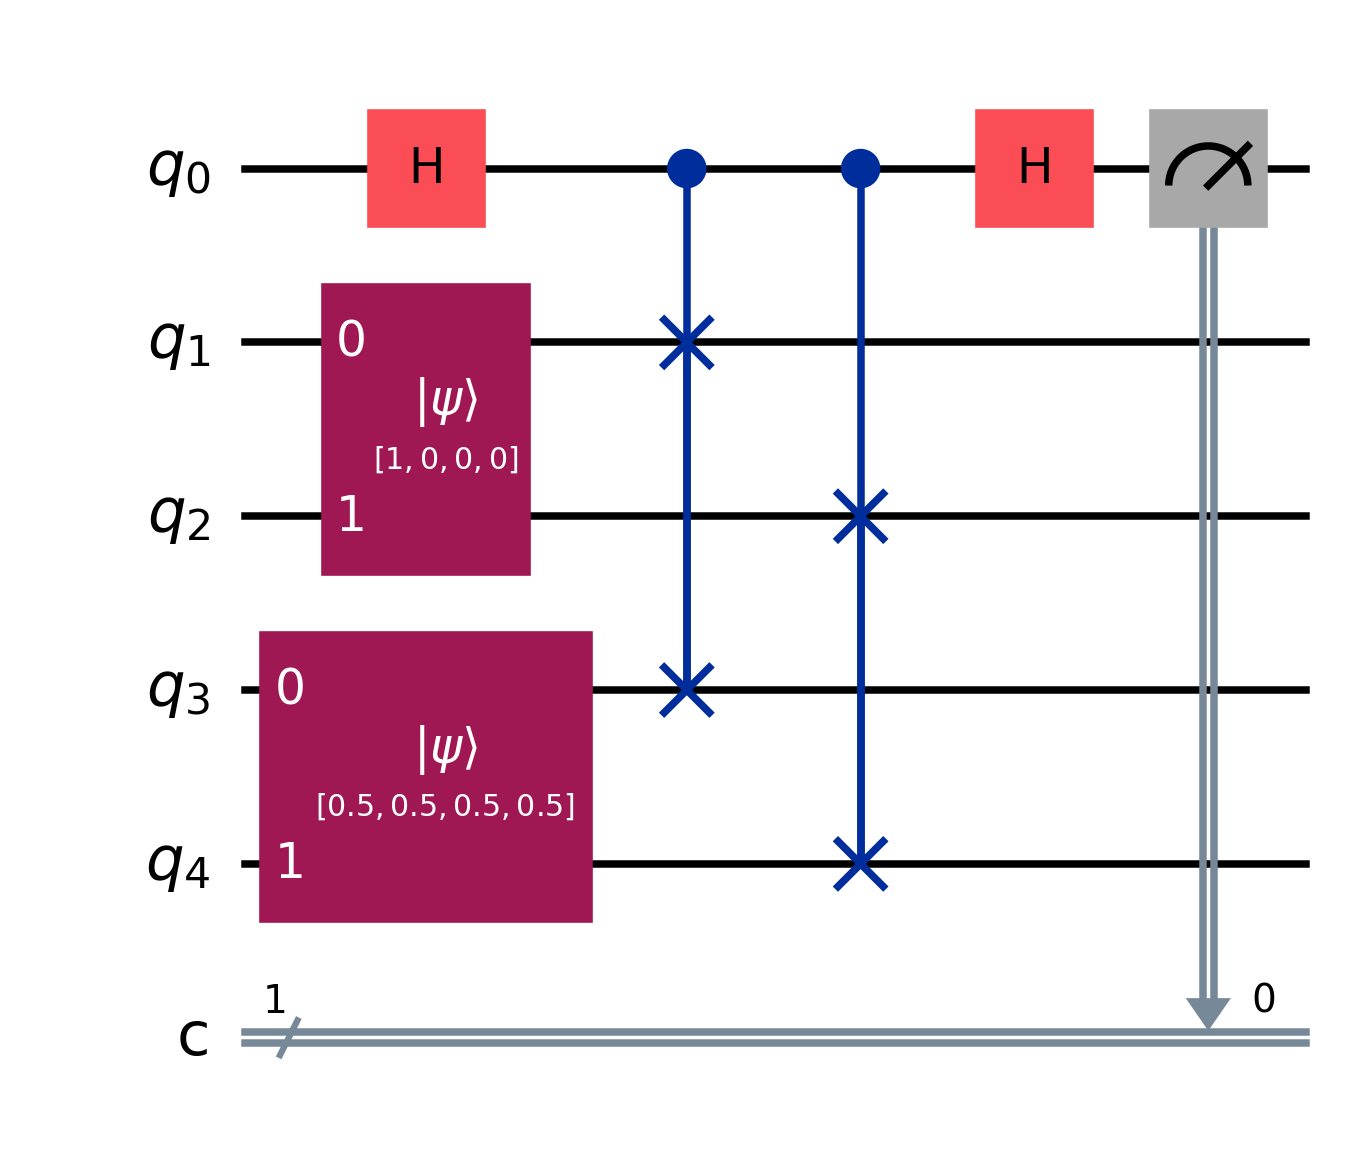
\includegraphics[width=0.7\linewidth]{figures/swap_test_circuit.png}
  \caption[Swap-test circuit]{Swap-test circuit for a four-dimensional example,
  in which each vector is amplitude-encoded into two qubits. The ancilla
  ($q_0$) is placed in superposition, controls a swap of the two encoded
  registers ($q_1 q_2$ and $q_3 q_4$), and is measured after a second Hadamard.
  The probability of reading the ancilla as zero gives the squared overlap of
  the two states, as in Equation~\ref{eq:swaptest}.}
  \label{fig:swaptest_circuit}
\end{figure}

\subsubsection{Qiskit Grover (Hardcoded Oracle)}
Grover's algorithm searches an unstructured collection of $N$ items for a marked
one using only about the square root of $N$ queries to an oracle, a quadratic
improvement over the $N$ comparisons a classical scan needs \cite{grover1996}.
Our engine implements the textbook circuit: it places an index register of
$\log_2 N$ qubits, with $N$ padded up to a power of two, into uniform
superposition, then repeats an oracle followed by a diffusion operator
$\lfloor\pi\sqrt{N}/4\rfloor$ times before measuring;
Figure~\ref{fig:grover_circuit} shows one such iteration for a four-element
index. The oracle flips the phase
of the target index and the diffusion step amplifies its amplitude, so the
measurement returns the marked index with high probability. The honest
difficulty is the oracle itself. For this to be a genuine search, the oracle
would have to compute, in superposition, which of the $N$ stored vectors is
closest to the query, which in turn requires loading all $N$ vectors into the
quantum state through a quantum random access memory, a device that addresses a
superposition of memory cells \cite{giovannetti2008qram}. No such hardware
exists at usable scale, and if instead the data has to be loaded one item at a
time the preparation alone costs $O(N)$, which erases the quadratic advantage
before the search even begins \cite{aaronson2015readfine}. We therefore make the
limitation explicit rather than hide it: the engine finds the nearest neighbour
classically and constructs an oracle that marks exactly that index. This
isolates the search step so that we can measure its oracle-call count and confirm
that it follows the $\lfloor\pi\sqrt{N}/4\rfloor$ curve, which is the scaling
claim we are actually testing, not an end-to-end speedup we are claiming to have
achieved.

\begin{figure}[ht]
  \centering
  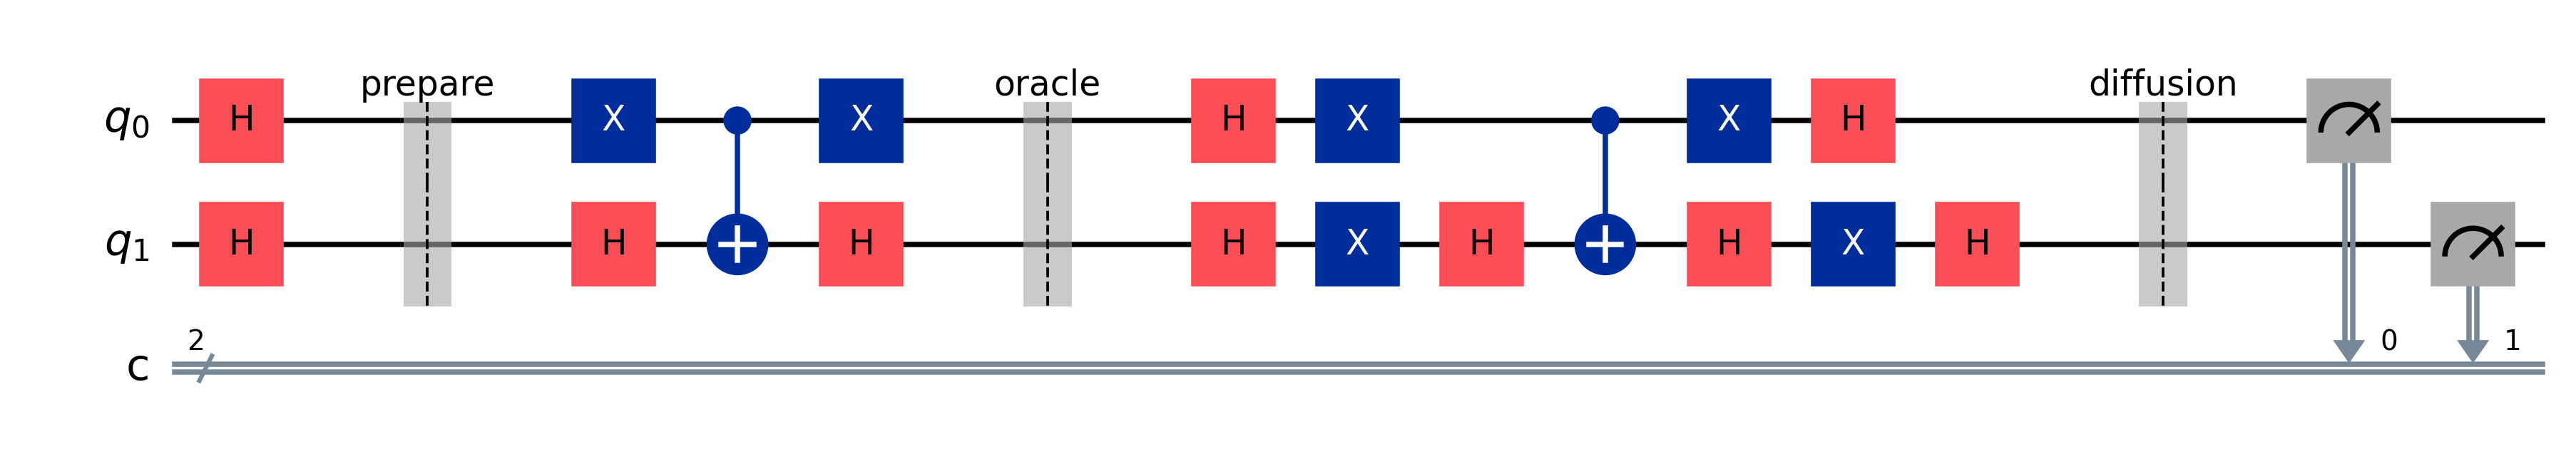
\includegraphics[width=\linewidth]{figures/grover_circuit.png}
  \caption[Grover circuit, one iteration]{One Grover iteration for a
  four-element index ($N=4$, two index qubits). After preparing a uniform
  superposition, the oracle flips the phase of the marked index and the
  diffusion operator amplifies its amplitude; the two qubits are then measured.
  The barriers separate the preparation, oracle, and diffusion phases.}
  \label{fig:grover_circuit}
\end{figure}

\subsubsection{Qiskit Grover with Quantum State Preparation}
The final Grover variant removes the one classical shortcut that the previous
engine kept. Instead of locating the nearest neighbour with a classical dot
product, it determines the target index quantum-mechanically: each stored vector
and the query are loaded with Qiskit state-preparation gates, a swap test
estimates their overlap, and the index with the highest measured overlap becomes
the one the Grover oracle marks. Everything after that, the superposition, the
oracle and diffusion iterations, and the final measurement, is identical to the
hardcoded variant. We include it to see what happens when the target selection
is itself made quantum, and therefore noisy, rather than exact. The outcome,
previewed here and quantified in the Results chapter, is that accuracy falls:
state preparation produces deep circuits, the per-candidate swap test carries the
same shot noise as the standalone swap-test engine, and any error in the quantum
target selection is then faithfully amplified by Grover, which has no mechanism
to recover once it has been pointed at the wrong index. This engine is thus the
most fully quantum of those we study and also the least accurate, a tension that
is itself one of the findings the project set out to document.

\subsubsection{Hybrid HNSW + Swap Test}
The hybrid engine is the one design in the study that tries to place the quantum
component where it might plausibly help rather than use it as a standalone
search. It runs in two stages. First the classical HNSW index retrieves a small
pool of candidates, by default the five nearest, cheaply narrowing the twenty
images down to a handful. The swap-test reranker then runs only on that pool,
scoring each surviving candidate against the query and reordering them. Because
the expensive quantum step is applied to a fixed-size shortlist instead of the
whole collection, the number of circuits no longer grows with the dataset: the
classical stage absorbs the $O(N)$ work and the quantum stage does a constant
amount of refinement on top. This mirrors the way approximate and exact stages
are already combined in production retrieval, where a fast approximate index
proposes candidates and a slower, more precise scorer reranks them, and it is the
most defensible place to insert a quantum estimator given that the swap test
offers no search speedup of its own. On our small collection the shortlist almost
always already contains the correct image, so the hybrid tracks the classical
baseline closely; its value here is architectural, showing the shape a useful
quantum contribution would take rather than a raw accuracy gain.

\subsubsection{IBM Hardware Validation}
To check that the quantum component is not merely a simulator artefact, we ran
the hybrid engine once on a real IBM quantum processor through the IBM Quantum
runtime, with the swap-test reranking executed on physical hardware rather than
the Aer simulator. This run is deliberately tiny. Vectors are truncated to just
two dimensions, the candidate pool is two images, and each circuit is measured
with thirty-two shots, a configuration small enough to fit within the limited
free-tier processor time and shallow enough that a noisy device can execute it at
all. It is a sanity check, not a scaling experiment: the aim is to confirm that
the encode, swap-test, and measure pipeline behaves on real hardware as it does
in simulation, and to expose honestly how much device noise and aggressive
truncation cost in accuracy. The resulting quality, reported with the other
measurements in the Results chapter, is far below the simulated engines and close
to chance, which is the expected consequence of two-dimensional vectors and
thirty-two shots on a noisy processor rather than a failure of the method. We
draw no scaling conclusions from it; its role is to ground the rest of the study,
which runs on a simulator, against at least one execution on a physical quantum
computer.

\section{Evaluation Metrics}
\label{sec:method:metrics}

% Define MRR formally, then define oracle calls. Explain why wall-clock is per-
% engine only - the simulator-time issue.

The primary measure of accuracy is the mean reciprocal rank (MRR), a standard
information-retrieval metric. For each query it rewards the engine with the
reciprocal of the rank at which the correct image appears: a correct image
ranked first scores one, ranked second one half, ranked fifth one fifth, and a
correct image that falls outside the top $k$ results returned, with $k$ fixed at
ten throughout, scores zero. Averaging this reciprocal rank over all queries
gives the MRR reported for an engine, as defined in Equation~\ref{eq:mrr}.
Because every engine is scored against the same ground-truth ranking and, as
established in Section~\ref{sec:method:embeddings}, the underlying similarity
measures induce identical orderings on unit vectors, a single MRR value can be
compared directly from one engine to the next.

\begin{equation}
\text{MRR} = \frac{1}{|Q|} \sum_{q \in Q} \frac{1}{\text{rank}_q},
\label{eq:mrr}
\end{equation}
where $\text{rank}_q$ is the position of the first relevant result for query
$q \in Q$ and $1/\text{rank}_q \coloneqq 0$ if no relevant result is in the top-$k$.

Accuracy alone does not capture why a quantum approach might ever be worth the
trouble, so we also record how each engine scales. The natural measure is the
operation count, the number of times an engine runs its core operation for a
single query, which is independent of the machine it runs on: a slow laptop and a
fast server execute the same number of iterations. The exhaustive engines, brute
force, FAISS flat, and the standalone swap test, perform one comparison or one
circuit per image and so scale as $O(N)$; HNSW traverses its graph in
$O(\log N)$; the hybrid does an $O(\log N)$ prefilter followed by a fixed number
$M$ of swap tests, $O(\log N + M)$; and Grover completes its search in
$\lfloor\pi\sqrt{N}/4\rfloor$ oracle cycles, $O(\sqrt{N})$. We store this figure
in the oracle-calls field of each result, and it is the only speed-like quantity
we compare across engines.

For the quantum engines we additionally record two circuit properties that
determine whether a circuit could run on real hardware. Circuit depth counts the
sequential layers of gates and is the main proxy for how much noise a physical
device would accumulate, since today's machines execute only a limited number of
layers reliably. Qubit count is the width of the circuit, which for the swap test
is the $1 + 2\lceil\log_2 d\rceil$ derived earlier. These fields are populated
only by the engines that build circuits; the classical engines leave them empty.
We deliberately do not compare wall-clock time across engines. The quantum
engines run on a simulator that reproduces quantum behaviour by manipulating an
exponentially large state vector on an ordinary CPU, so their runtimes mostly
measure the cost of that simulation rather than anything intrinsic to the
algorithm; comparing them with classical CPU timings would penalise the quantum
methods for the wrong reason. We therefore report wall-clock only within a single
engine, where it is meaningful, and never as a cross-engine ranking.

\section{Experimental Configuration}
\label{sec:method:config}

Table~\ref{tab:config} lists the parameter grid the benchmark sweeps. The
harness runs the full cartesian product of these values: every engine is
evaluated at each vector dimension, and the four quantum engines, which accept a
shot count, are additionally run at each shot setting, while the three classical
engines ignore shots and are run once per dimension. Each resulting
configuration is evaluated on all twenty queries. This produces fifteen
engine-and-shot configurations per dimension, three classical and four quantum at
three shot counts each, forty-five across the three dimensions, and nine hundred
individual query runs once multiplied by the twenty queries. The separate IBM
hardware validation contributes a further twenty runs, one per query, for a
stored total of nine hundred and twenty results. The layers parameter is held at
one throughout; the harness requires it but no engine enabled here uses it. Every
run is written to a PostgreSQL table together with its full parameter set, and
the database is dumped to a seed file committed alongside the code, so the entire
dataset can be reconstructed exactly rather than trusted as a one-off snapshot.

\begin{table}[ht]
  \centering
  \caption{Benchmark configuration grid.}
  \label{tab:config}
  \begin{tabular}{l p{7.2cm}}
    \toprule
    \textbf{Parameter} & \textbf{Values} \\
    \midrule
    Engines             & Brute-force cosine, FAISS flat, FAISS HNSW
                          (classical); swap test, Grover (hardcoded oracle),
                          Grover (quantum prep), hybrid HNSW + swap test
                          (quantum) \\
    Dimensions          & 64, 128, 256 \\
    Shots               & 512, 1024, 2048 (quantum engines only) \\
    Layers              & 1 \\
    Top-$k$             & 10 \\
    \bottomrule
  \end{tabular}
\end{table}

\section*{Use of AI Tools}
\label{sec:method:ai}
\addcontentsline{toc}{section}{Use of AI Tools}

% MANDATORY per FENS handbook \S1.1. Be specific - generic disclaimers fail
% the originality check. State which tools were used for which tasks.

This project made use of AI assistants, specifically Claude Code and ChatGPT, as
productivity tools during development and writing. Their role was to accelerate
well-defined, labour-intensive tasks under the authors' direction, not to
originate the work. Concretely, the tools assisted with generating and
refactoring routine code, reviewing changes and helping locate bugs during the
code audit, drafting prose that the authors then revised, and rendering diagrams
from layouts the authors specified.

The intellectual core of the project is the authors' own. The system
architecture, including the strategy-pattern engine interface and the five-phase
pipeline, the selection and configuration of the search engines, the design of
the benchmark and its research questions, and the interpretation of the results
were reasoned through and decided by the authors. Every benchmark figure reported
here was produced by our own experimental runs, and every external reference was
verified by the authors against its primary source before it was cited.

The authors take full responsibility for the correctness, originality, and
verification of all code, data, and conclusions in this report. Where AI tools
contributed text or code, that output was read, checked, and where necessary
corrected and rewritten by the authors, who treat it as a draft to be
scrutinised rather than as an authority to be trusted.

\chapter{RESULTS AND ANALYSIS}
\label{ch:results}

% State main findings in words FIRST, then go into details. Use subheadings.
% Every claim here must be backed by a row in benchmark_results or a figure
% generated from it. No prose claims without a number behind them.
% Target length: ~1,500-2,500 words.

In the noiseless simulator benchmark, retrieval accuracy mainly depended on the
embedding dimension, not on whether the engine was classical or quantum. The
three classical baselines returned identical rankings and tied at MRR 0.829, and
every engine improved as the dimension rose from 64 to 256. The swap test
reproduced the classical ranking at dimension 256 (MRR 0.975) and recovered at
lower dimensions as shots increased. Grover with a hardcoded oracle matched the
theoretical $\lfloor(\pi/4)\sqrt{N}\rfloor$ oracle count, but its probabilistic
measurement stopped at MRR 0.955 at dimension 256. Grover with quantum state
preparation was weakest (MRR 0.559). The hybrid engine effectively tied the
classical baseline (MRR 0.823) by using HNSW for search and the swap test only
for reranking.

These accuracy results should not be read as predictions for a large, noisy
quantum computer. The simulator removes gate noise, measurement error beyond
finite-shot sampling, queueing, and hardware latency. The measured pattern still
answers the algorithmic question under controlled conditions, but real hardware
would be expected to degrade the quantum-engine accuracy unless error rates and
circuit depth are low enough for the chosen workload.

\section{Accuracy Across Engines}
\label{sec:results:mrr}

% MRR per engine, broken out by dimension and shots where relevant. Use the
% same table layout as the frontend BenchmarkResults component.

\begin{table}[ht]
  \centering
  \caption[Mean Reciprocal Rank by engine and dimension]{Average Mean
  Reciprocal Rank (MRR) by engine and embedding
  dimension, over the twenty benchmark queries. Higher is better: an MRR of
  1.000 means the correct image was ranked first for every query. Quantum
  cells average over the three shot counts (512, 1024, 2048); the shot
  dependence is examined separately below. The IBM hardware run is reported
  in Section~\ref{sec:results:ibm}.}
  \label{tab:mrr}
  \begin{tabularx}{\linewidth}{Xcccc}
    \toprule
    & \multicolumn{3}{c}{\textbf{MRR by dimension}} & \\
    \cmidrule(lr){2-4}
    \textbf{Engine} & \textbf{64} & \textbf{128} & \textbf{256} & \textbf{Avg} \\
    \midrule
    Brute-force cosine          & 0.655 & 0.858 & 0.975 & 0.829 \\
    FAISS flat                  & 0.655 & 0.858 & 0.975 & 0.829 \\
    FAISS HNSW                  & 0.655 & 0.858 & 0.975 & 0.829 \\
    \addlinespace
    Swap test                   & 0.470 & 0.738 & 0.975 & 0.728 \\
    Grover (hardcoded oracle)   & 0.546 & 0.776 & 0.955 & 0.759 \\
    Grover (quantum state prep) & 0.404 & 0.551 & 0.722 & 0.559 \\
    \addlinespace
    Hybrid (HNSW + swap test)   & 0.635 & 0.858 & 0.975 & 0.823 \\
    \bottomrule
  \end{tabularx}
\end{table}

Table~\ref{tab:mrr} shows that brute-force cosine, FAISS flat, and FAISS HNSW
all scored MRR 0.829 and produced the same query-by-query ordering. This is
expected: brute force and FAISS flat are exact searches over the same twenty
unit vectors, and HNSW's approximation does not matter on a graph this small. We
treat the brute-force result as the reference ordering.

Embedding dimension had the strongest effect on accuracy. Every engine improved
from dimension 64 to 256, and the classical baseline moved through 0.655, 0.858,
and 0.975. Truncating CLIP vectors discards information that separates
near-neighbours; restoring dimensions recovers it. The lower dimensions are
therefore a simulation trade-off, not the configuration a retrieval system would
prefer.

The swap test illustrates how a quantum estimator approaches the exact answer as
its measurement budget grows. At dimension 256 it matched the best classical
score exactly (MRR 0.975 at every shot count), because the overlaps it estimates
are well separated and even a coarse estimate ranks them correctly. At dimension
128, where neighbours are closer together, accuracy depended on how finely we
measured: MRR rose from 0.642 at 512 shots to 0.688 at 1024 and 0.883 at 2048.
The swap test estimates the squared overlap $|\langle\psi|\phi\rangle|^2$ from
a finite number of measurements, so additional shots reduce the sampling noise
and sharpen the ranking. This shot-versus-accuracy trade-off, rather than a
fixed limit of the method itself, explains the swap test's lower average of
0.728: the average is pulled down by the low-dimension, low-shot configurations
that a practical deployment would not choose.

The two Grover engines separate sharply. The hardcoded-oracle version reached
MRR 0.955 at dimension 256, just short of the best classical score of 0.975,
because the marked state is still measured probabilistically. The quantum
state-preparation variant was weakest at every dimension and averaged 0.559:
state preparation and
per-candidate swap tests add noise before Grover amplifies the chosen index. The
hybrid takes the opposite approach. HNSW chooses the candidates, and the swap
test reranks only that shortlist, so it stayed close to the baseline (MRR 0.823,
and 0.975 at dimension 256).

\section{Quantum Resource Cost}
\label{sec:results:cost}

% Circuit depth, qubit count, oracle calls. This section answers RQ2 (Grover
% scaling) and supports the practicality framing on RQ3.

Because the quantum engines run on a classical simulator, their wall-clock time
measures simulation overhead rather than the cost of a real quantum device
(Section~\ref{sec:results:walltime} returns to this). The hardware-neutral way
to compare the engines is therefore to count the operations each one performs per
query and the resources its circuit would demand on a real device.
Table~\ref{tab:opcount} reports the first of these: the number of similarity
comparisons or oracle calls each engine makes for a single query over the
twenty-image dataset.

\begin{table}[ht]
  \centering
  \caption[Operations per query and complexity class]{Operations per query and
  algorithmic complexity for each engine over
  the twenty-image dataset ($N=20$). The operation count is the cross-engine
  scaling metric; it is independent of hardware. Here $M$ denotes the number of
  candidates the hybrid engine reranks.}
  \label{tab:opcount}
  \begin{tabularx}{\linewidth}{Xcc}
    \toprule
    \textbf{Engine} & \textbf{Operations / query} & \textbf{Complexity} \\
    \midrule
    Brute-force cosine          & 20 & $O(N)$ \\
    FAISS flat                  & 20 & $O(N)$ \\
    FAISS HNSW                  & 5  & $O(\log N)$ approx. \\
    \addlinespace
    Swap test                   & 20 & $O(N)$ \\
    Grover (hardcoded oracle)   & 4  & $O(\sqrt{N})$ \\
    Grover (quantum state prep) & 4  & $O(\sqrt{N})$ \\
    \addlinespace
    Hybrid (HNSW + swap test)   & 10 & $O(\log N + M)$ \\
    \bottomrule
  \end{tabularx}
\end{table}

Grover was the only engine whose per-query cost was sublinear in the dataset
size. The exact classical engines and the standalone swap test each performed one
comparison per stored vector, twenty in total, while FAISS HNSW reached its
answer in about five graph hops and the hybrid engine made ten comparisons (one
HNSW shortlist followed by a swap-test rerank of the survivors). Both Grover
engines used four oracle calls, and this count is exactly what the theory
predicts once the index padding is accounted for. Grover addresses an index
register whose length is a power of two, so the twenty images are padded to the
next power of two, $N' = 32$, which is why the Grover circuits used five qubits
($\lceil \log_2 32 \rceil = 5$). The optimal number of Grover iterations for an
unstructured search of $N'$ items is $\lfloor (\pi/4)\sqrt{N'} \rfloor$, and for
$N' = 32$ this evaluates to $\lfloor 4.44 \rfloor = 4$, matching the measured
count. Figure~\ref{fig:oracle_scaling} places this verified point on the
theoretical curve.

\begin{figure}[ht]
  \centering
  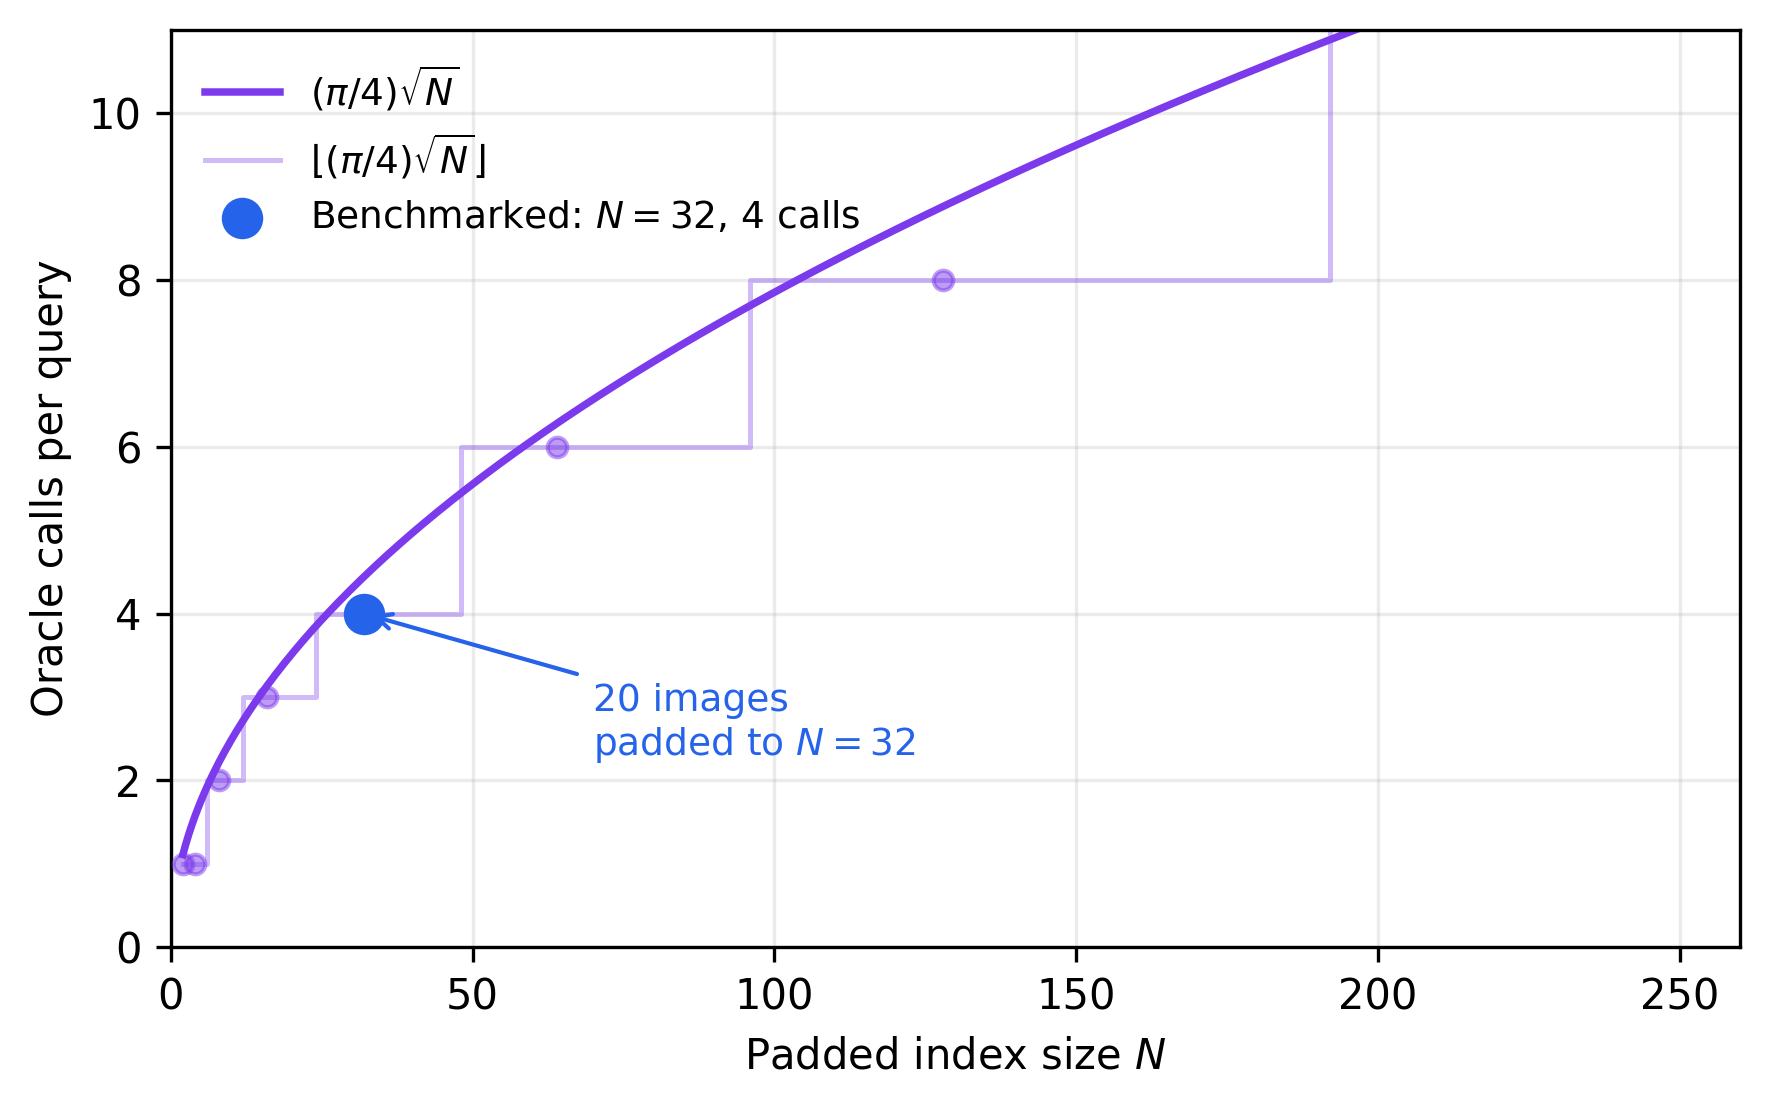
\includegraphics[width=0.8\linewidth]{figures/oracle_scaling.png}
  \caption[Grover oracle-call scaling]{Theoretical Grover oracle-call count
  $\lfloor (\pi/4)\sqrt{N} \rfloor$ as a function of the padded index size $N$,
  with a marker at the single size we benchmarked ($N = 32$, four oracle calls).
  We ran one dataset size, so this confirms the count at a single point on the
  curve rather than tracing the curve empirically.}
  \label{fig:oracle_scaling}
\end{figure}

The two quantum families differ sharply in what they encode, and
Table~\ref{tab:circuitcost} shows the consequence for circuit width and depth.
Grover encodes the candidate \emph{index}, so its width stayed fixed at five
qubits regardless of the embedding dimension; its cost instead appears as depth,
around fifty gate layers, because each of the four iterations applies an oracle
and a diffusion operator in sequence. The swap test and the hybrid engine encode
the candidate \emph{vectors}, so their width grew with the embedding dimension as
$1 + 2\lceil \log_2 d \rceil$ qubits, from thirteen at dimension 64 to seventeen
at dimension 256, while their circuits stayed shallow (depth nine to eleven). On
near-term hardware both costs matter: more qubits are harder to allocate, and
greater depth gives decoherence more time to corrupt the state, which is the
practical reason the deep Grover circuits would be the harder of the two to run
faithfully on a real device.

\begin{table}[ht]
  \centering
  \caption[Quantum circuit width and depth]{Circuit width and depth for the
  quantum engines, from the compiled
  circuits. The swap test and the hybrid engine share the same circuit metrics
  because the hybrid reuses the swap-test circuit. Grover's width is set by the
  padded index register, not the embedding dimension, so it is constant.}
  \label{tab:circuitcost}
  \begin{tabularx}{\linewidth}{Xccc}
    \toprule
    \textbf{Engine (dimension)} & \textbf{Qubits} & \textbf{Circuit depth} \\
    \midrule
    Swap test / Hybrid, dim 64   & 13 & 9 \\
    Swap test / Hybrid, dim 128  & 15 & 10 \\
    Swap test / Hybrid, dim 256  & 17 & 11 \\
    \addlinespace
    Grover (both variants), any dim & 5 & $\approx 50$ \\
    \bottomrule
  \end{tabularx}
\end{table}

These counts also expose the assumption hidden inside Grover's sublinear figure.
The four oracle calls measure only the search once the data is already encoded in
the oracle; they do not include the cost of building that oracle. Our hardcoded
oracle computes the nearest neighbour classically and then marks it, so the
twenty comparisons Grover appears to save have in effect been paid before the
circuit runs. This is the qRAM caveat set out in Section~\ref{sec:method:engines}:
a genuine quantum speed-up for search would require loading the dataset into a
quantum-accessible memory, which is itself an unsolved cost. The swap test and
hybrid engines make the opposite trade, paying their cost openly in qubits and in
one circuit execution per candidate. Section~\ref{sec:results:discussion} returns
to what this means for the practicality question.

\section{Wall-Clock Behaviour (Within-Engine Only)}
\label{sec:results:walltime}

% IMPORTANT: per docs/NOTES.md, wall-clock is NOT a valid cross-engine metric on
% a simulator. State this in the first sentence to avoid the reader misreading
% the numbers.

Wall-clock time cannot be compared across engines in this study, and
Table~\ref{tab:walltime} should be read only one row at a time. The reason is
that the quantum engines did not run on a quantum computer: they ran on a
classical statevector simulator, which represents the full quantum state in
ordinary memory and so does work that grows exponentially with the number of
qubits. The times for the quantum engines therefore measure the cost of
\emph{simulating} a circuit on a CPU, not the latency a real quantum processor
would incur, and putting them next to the classical millisecond figures would
compare two unrelated quantities. The within-engine comparison across dimension
is meaningful, because there the hardware is held fixed and only the problem size
changes.

\begin{table}[ht]
  \centering
  \caption[Mean query time by engine and dimension]{Mean total time per query,
  in milliseconds, by engine and embedding
  dimension. The three classical engines completed in well under a millisecond
  (0.2 to 0.6 ms) and are shown as ``$<1$''. The quantum and hybrid times are
  simulator times on a CPU and are \emph{not} comparable to the classical
  figures or to real quantum hardware; they are reported only to show how each
  engine's simulation cost scales with dimension.}
  \label{tab:walltime}
  \begin{tabularx}{\linewidth}{Xccc}
    \toprule
    & \multicolumn{3}{c}{\textbf{Mean time per query (ms)}} \\
    \cmidrule(lr){2-4}
    \textbf{Engine} & \textbf{dim 64} & \textbf{dim 128} & \textbf{dim 256} \\
    \midrule
    Brute-force cosine          & $<1$ & $<1$  & $<1$ \\
    FAISS flat                  & $<1$ & $<1$  & $<1$ \\
    FAISS HNSW                  & $<1$ & $<1$  & $<1$ \\
    \addlinespace
    Swap test                   & 993  & 4764  & 21555 \\
    Grover (hardcoded oracle)   & 19   & 20    & 19 \\
    Grover (quantum state prep) & 3399 & 6916  & 7453 \\
    Hybrid (HNSW + swap test)   & 254  & 1134  & 5255 \\
    \bottomrule
  \end{tabularx}
\end{table}

Read row by row, the table reflects circuit size. The swap test and hybrid
slowed sharply as dimension rose, because each doubling adds two qubits to the
amplitude encoding and quadruples the simulator state. The swap test grew from
about one second per query at dimension 64 to roughly twenty-two seconds at
dimension 256. Hardcoded Grover stayed near twenty milliseconds because it uses
the same five-qubit index register at every dimension. The simulator, not the
algorithm, set the cap of 256 dimensions.

\section{IBM Hardware Sanity Check}
\label{sec:results:ibm}

% The dimension-2, 2-candidate validation run. Frame as: "we want to confirm
% the swap test circuit behaves the same on real hardware as on the simulator,
% within shot noise". Do NOT make scaling claims from this.

All of the quantum results above were produced on a simulator. To confirm that
the swap-test pipeline also runs on a physical quantum processor, we executed the
hybrid engine once on real IBM Quantum hardware through the IBM Quantum cloud
service. This run was deliberately tiny: it used two-dimensional vectors, two
candidates per query, and thirty-two measurement shots, across the same twenty
queries, and it consumed eighty seconds of the limited free-tier quota. We treat
it as a sanity check on the execution path, not as a benchmark, and it is kept
separate from the simulator results for that reason.

The run achieved MRR 0.125, far below the simulator figures. This reflects the
configuration rather than the method: two-dimensional vectors remove most
semantic information, two candidates make the task close to a coin toss, and
thirty-two shots give a noisy overlap estimate before device noise is added. The
run establishes only that the hardware path works end to end. It does not
support accuracy or scaling claims.

\section{Discussion}
\label{sec:results:discussion}

% Tie results back to the three research questions. Answer each one explicitly:
% "RQ1: yes, swap test reproduces classical ranking at >= X shots. RQ2: yes,
% oracle count matches theory to within Y%. RQ3: no - HNSW beats Grover even
% under ideal-qRAM assumptions at N >= Z."

\textbf{RQ1 (Accuracy).} The swap test reproduced the retrieval accuracy of
classical cosine similarity once it was given enough measurement shots, and the
shot budget it needed depended on how close the candidate vectors were. At
dimension 256, where neighbours are well separated, it matched the classical MRR
of 0.975 at every shot count we tried, including the smallest. At dimension 128
it reached classical accuracy only at the highest setting, rising to 0.883 at
2048 shots from 0.642 at 512, and at dimension 64 it remained below the classical
baseline even at 2048 shots. The pattern is consistent with the swap test being a
sampled estimate of vector overlap: the harder the discrimination, the more shots
are required to resolve it. \emph{Yes: the swap test reproduces classical
retrieval accuracy given a sufficient shot budget, and the budget required grows
as the embedding dimension, and hence the separation between neighbours, falls.}

\textbf{RQ2 (Scaling).} Our Grover implementation used four oracle calls per
query, which is exactly the theoretical optimum $\lfloor (\pi/4)\sqrt{N'}
\rfloor$ for the padded index size $N' = 32$, as set out in
Section~\ref{sec:results:cost}. The match was exact rather than approximate.
The qualification is that we benchmarked only one dataset size, so we confirmed
the formula at a single point rather than tracing the scaling curve across a
range of $N$. \emph{Yes: at the size we tested, the oracle-call count matched the
theoretical $\lfloor (\pi/4)\sqrt{N} \rfloor$ optimum exactly, though a single
dataset size cannot demonstrate the full curve.}

\textbf{RQ3 (Practicality).} No engine that performed the search on a quantum
circuit beat the classical HNSW baseline on this dataset. HNSW reached the full
brute-force accuracy of 0.829 in about five graph hops, while the standalone
quantum engines were either less accurate or, in Grover's case, dependent on a
classically precomputed oracle. The one quantum-containing engine that matched
the baseline, the hybrid, did so precisely because the classical index performed
the search and the swap test only reranked a shortlist; its accuracy is inherited
from HNSW, not produced by the quantum step. \emph{We found no condition under
which a quantum search engine outperformed the HNSW baseline on this dataset; the
strongest quantum-containing engine matched it only by delegating the search
itself to the classical index.}

\textbf{RQ4 (Fit).} The resource accounting in
Section~\ref{sec:results:cost} points to a reason for the RQ3 result.
Grover's sublinear oracle count is genuine, but it measures the search after the
data has been loaded into the oracle; constructing that oracle, or an equivalent
quantum-accessible memory, reintroduces a cost linear in the dataset size. Vector
retrieval is dominated by exactly this data-loading step, because answering a
query means comparing against many stored items. Quantum advantage, by contrast,
is generally argued to concentrate on compute-bound problems that do heavy
processing over small inputs rather than on data-bound problems that must read a
large dataset~\cite{aaronson2015readfine,hoefler2023practicality}. \emph{On both
our evidence and the structure of the problem, the search part of cross-modal
vector retrieval is not a good match for quantum advantage under the methods we
tested. A quantum step is more plausible as a reranker for a small shortlist than
as the engine that scans or indexes the whole dataset.}

\section{Limitations}
\label{sec:results:limitations}

% Be honest. Small dataset (20 images), simulator-only quantum execution,
% truncated CLIP embeddings, classical-precomputed Grover oracle.

Several constraints bound the results. The dataset has twenty images and one
query per image, which kept the sweep simulable and the target unambiguous but
limited statistical power. HNSW did not have enough vectors to exercise its
approximation, so its match with exact search holds only here. Except for the
IBM sanity check, the quantum engines ran on a classical simulator, so the
results do not measure present-day hardware noise or latency. Embeddings were
truncated from 512 to at most 256 dimensions to fit the qubit budget, so absolute
MRR values are comparisons under a shared handicap. Grover used a classically
precomputed oracle, and its oracle-call scaling was checked at one dataset size,
not across a range.

\chapter{SUSTAINABILITY, INCLUSIVITY, AND SOCIETAL IMPACT}
\label{ch:sustainability}

% Short reflection (one or two paragraphs is enough per template). SDG mapping
% optional. The poster grading form awards up to +10% bonus for this, so worth
% getting right.

This project was designed to be modest in its use of resources. The quantum
engines ran on a CPU-based circuit simulator over a deliberately small dataset of
twenty images, rather than on large-scale GPU training or extended
quantum-hardware time, so the entire benchmark sweep completes on a single
workstation; the one run on real quantum hardware consumed eighty seconds of a
free-tier quota. The data raises no privacy concerns, as Flickr30k is a public
research dataset of captioned images and contains no personal identifying
information that we collect or process. The work is openly reproducible: the
source code, the benchmark harness, and the dataset configuration are publicly
available, and the harness is deterministic, so the reported results can be
regenerated from scratch.

Beyond these practical points, the study makes a small contribution to how
quantum computing is discussed. Public accounts often present quantum advantage
as imminent and general; by measuring where quantum search helps and where it
does not, and by being explicit about the data-loading cost that the headline
speed-ups omit, the work offers a counterweight to that framing. In the language
of the United Nations Sustainable Development Goals, the project speaks most
directly to SDG~4 (quality education), as an openly available teaching artefact
for quantum and classical retrieval, and to SDG~9 (industry, innovation, and
infrastructure), as an honest assessment of a candidate technology's readiness.

\chapter{CONCLUSION}
\label{ch:conclusion}

% Summarise findings, highlight contributions, point to future work.
% Target length: ~300-500 words. No new results may appear here.

[SUMMARY \,--\, restate the three research questions and their answers in two
to three sentences.]

[CONTRIBUTIONS \,--\, list what this work delivered: (1) the benchmark
infrastructure, (2) the empirical verification of swap-test and Grover
behaviour, (3) the web application for inspection, (4) the honest analysis of
where the quantum-classical gap actually lies. The honest framing IS a
contribution - say so.]

[FUTURE WORK \,--\, candidates: larger dataset (Flickr30k full set or
ImageNet subset), wider dimension sweep (256, 512), proper variational ansatz
study, comparison against pgvector HNSW as a third classical baseline, IBM
hardware noise characterisation.]


% ============================  BACK MATTER  ==================================
\cleardoublepage
\addcontentsline{toc}{chapter}{REFERENCES}
\bibliography{references}

\appendix
\chapter{APPENDICES}
\label{ch:appendix}
\addcontentsline{toc}{chapter}{APPENDICES}

% Optional. Use for material too long to fit in the body but worth including
% for completeness. Candidates listed below - drop the ones we choose not to
% include.

\section*{Appendix A: Engine Configuration File}
[Reproduce backend/config/benchmarks.yaml verbatim with a \texttt{lstlisting}
block.]

\section*{Appendix B: Database Schema}
[Reproduce the benchmark\_results table definition from db/migrations.]

\section*{Appendix C: Repository}
[Link to the public GitHub repository and tag of the report-version commit.]


\end{document}
